\section{Measuring Equilibrium Mean Values of the Observables}
We now run the simulation for the same three temperatures ${0.3, 1.0, 2.0}$ including random particle positions and the previously described warm up. We run the simulations for 1200 time steps. Using our command line arguments an example looks like:

{\tt python ljsim.py --warm 20 --tstat 0.3 --time 120}

This sets an inital force cap of 20. The equilibration of the observables is plotted in the following figures with the first 100 timesteps omitted to preserve plot scaling. The command to produce these plots with our command line arguments looks like:

{\tt python ljanalyze.py --datafile ../dat/ljsim\_T2d0\_F20d0.dat --tlim 100 1199 --M 100}

Here we used a window of $M = 100$.
\begin{figure}[ht]
\begin{subfigure}{0.3\textwidth}
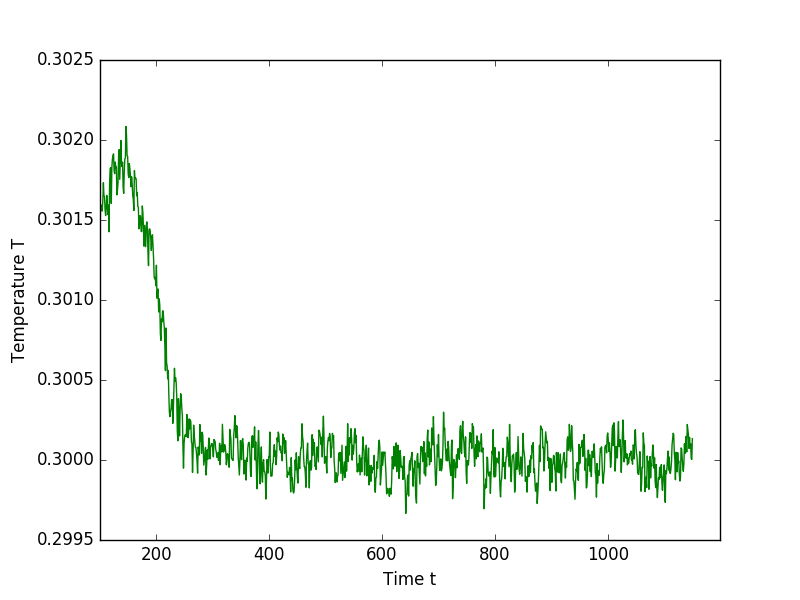
\includegraphics[width=\textwidth]{fig/avTemperature_T0d3_F20d0_M100.png}
\end{subfigure}
\hfill
\begin{subfigure}{0.3\textwidth}
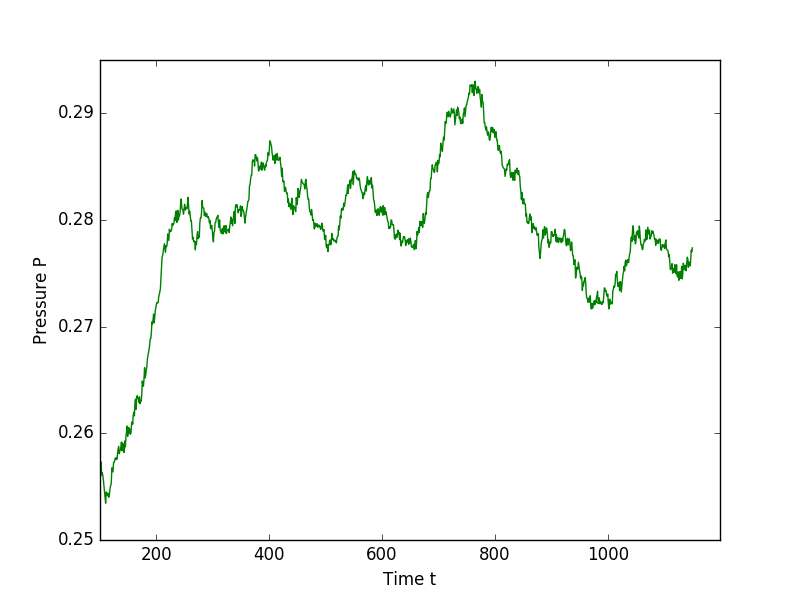
\includegraphics[width=\textwidth]{fig/avPressure_T0d3_F20d0_M100.png}
\end{subfigure}
\hfill
\begin{subfigure}{0.3\textwidth}
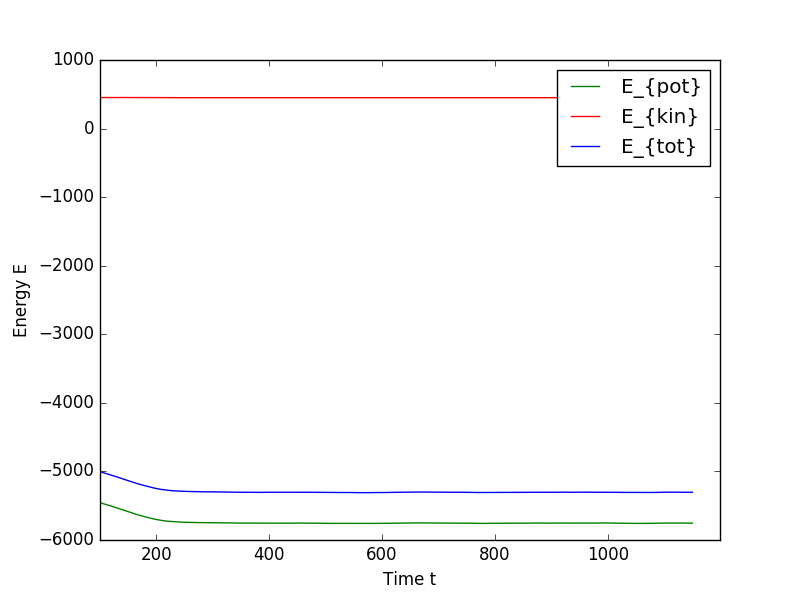
\includegraphics[width=\textwidth]{fig/avEnergies_T0d3_F20d0_M100.png}
\end{subfigure}
\end{figure}

\begin{figure}[ht]
\begin{subfigure}{0.3\textwidth}
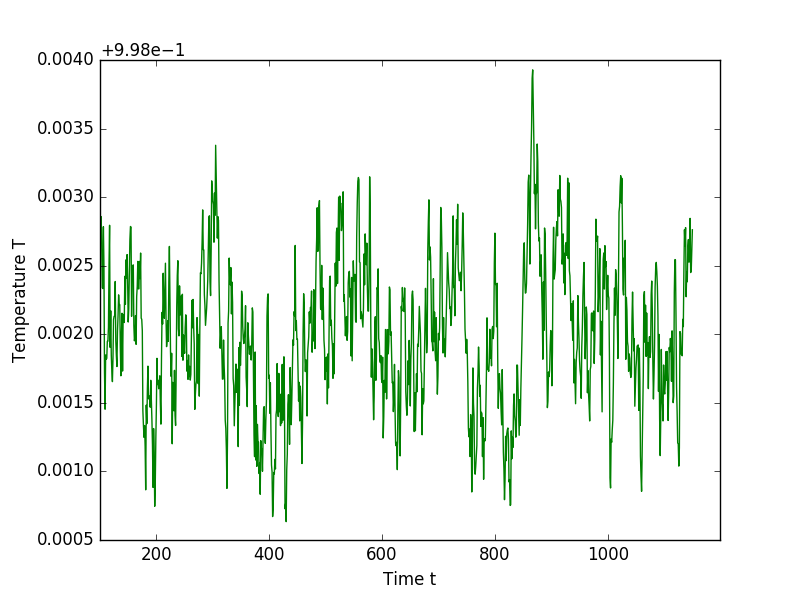
\includegraphics[width=\textwidth]{fig/avTemperature_T1d0_F20d0_M100.png}
\end{subfigure}
\hfill
\begin{subfigure}{0.3\textwidth}
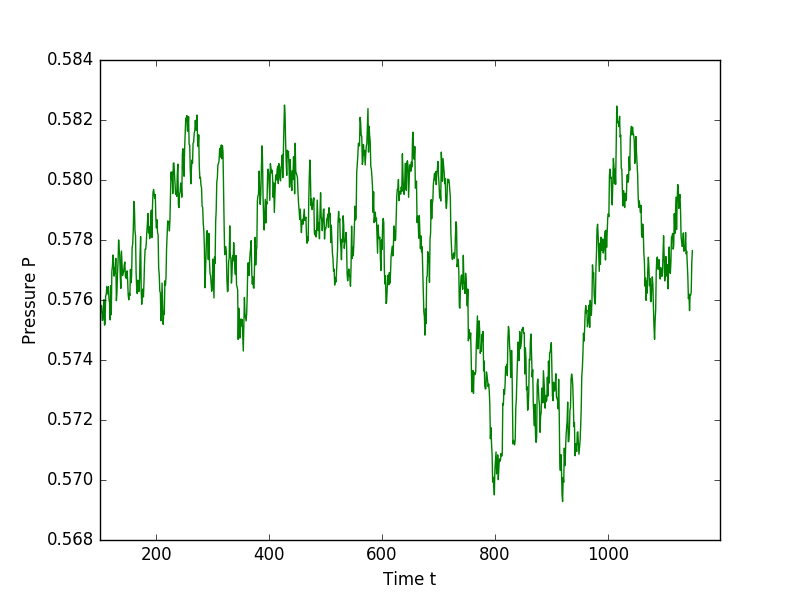
\includegraphics[width=\textwidth]{fig/avPressure_T1d0_F20d0_M100.png}
\end{subfigure}
\hfill
\begin{subfigure}{0.3\textwidth}
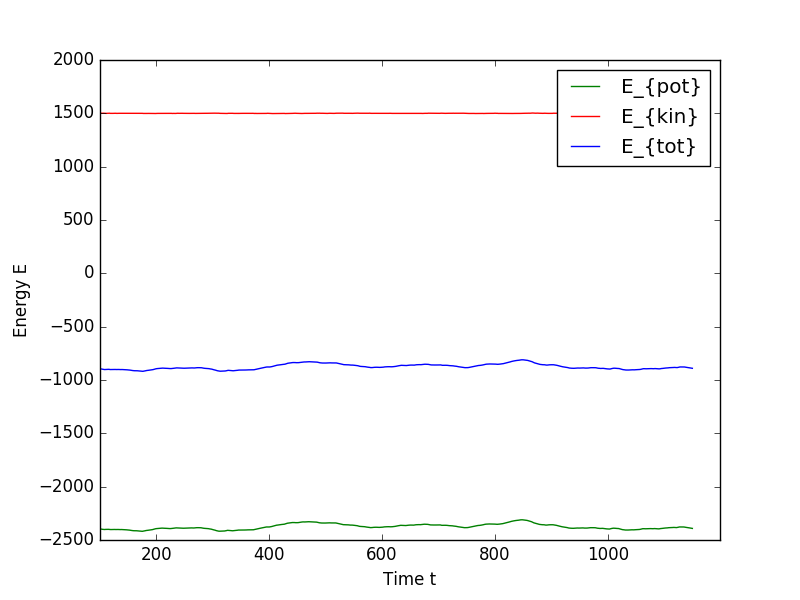
\includegraphics[width=\textwidth]{fig/avEnergies_T1d0_F20d0_M100.png}
\end{subfigure}
\end{figure}

\begin{figure}[ht]
\begin{subfigure}{0.3\textwidth}
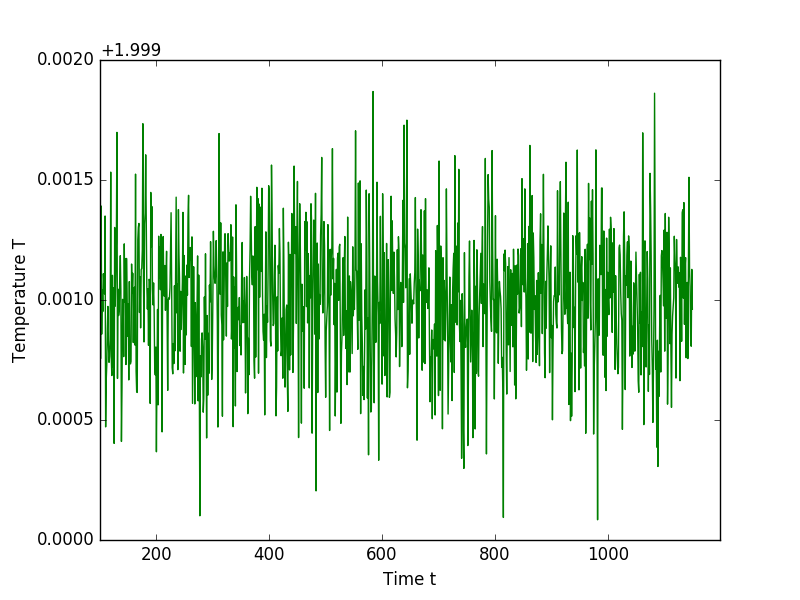
\includegraphics[width=\textwidth]{fig/avTemperature_T2d0_F20d0_M100.png}
\end{subfigure}
\hfill
\begin{subfigure}{0.3\textwidth}
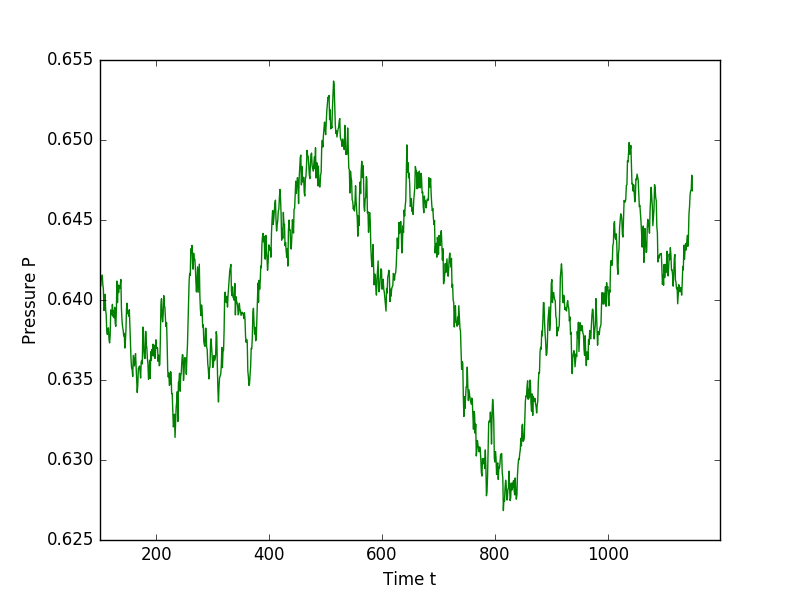
\includegraphics[width=\textwidth]{fig/avPressure_T2d0_F20d0_M100.png}
\end{subfigure}
\hfill
\begin{subfigure}{0.3\textwidth}
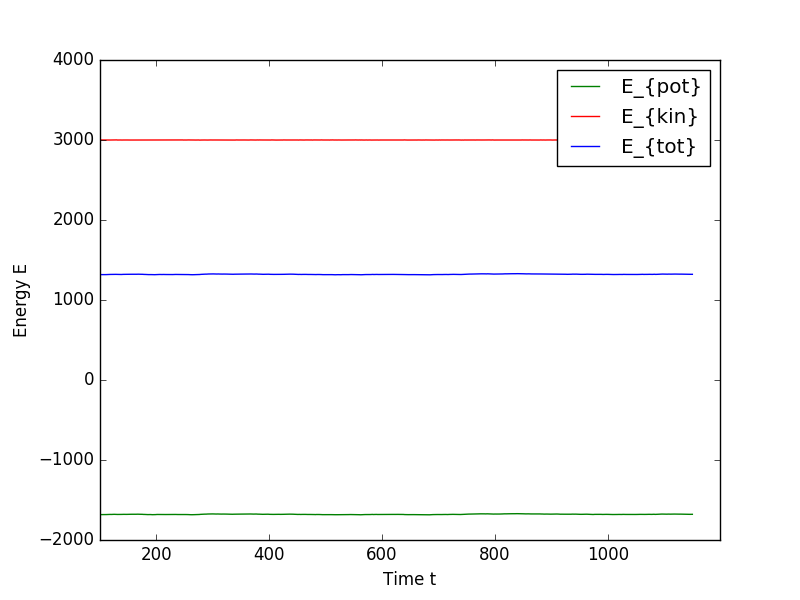
\includegraphics[width=\textwidth]{fig/avEnergies_T2d0_F20d0_M100.png}
\end{subfigure}
\end{figure}

The commands only differed in the thermostat temperature and the datafilename to be analyzed. Finally we plot the average RDF for the three different temperatures after equilibrium and compute the mean equilibrium values of the observables. The command to perform this analysis is:

{\tt python ljanalyze.py --datafile ../dat/ljsim\_T0d3\_F20d0.dat --teq 400}

\noindent Here we have assumed that our system has equilibrated by timestep 400. For $T = 0.3$ we measured $E_\mathrm{pot} = -5754.9$, $E_\mathrm{kin} = 450.0$, $E_\mathrm{tot} = -5304.9$, $T = 0.300$, and $P = 0.281$. For  $T = 1.0$ we measured $E_\mathrm{pot} = -2367.3$, $E_\mathrm{kin} = 1500.1$, $E_\mathrm{tot} = -867.3$, $T = 1.000$, and $P = 0.577$. For $T = 2.0$ we measured $E_\mathrm{pot} = -1679.0$, $E_\mathrm{kin} = 3000.0$, $E_\mathrm{tot} = 1321.0$, $T = 2.000$, and $P = 0.642$. The equilibruim RDF plots follow with temperature increasing from left to right.

\begin{figure}[ht]
\begin{subfigure}{0.3\textwidth}
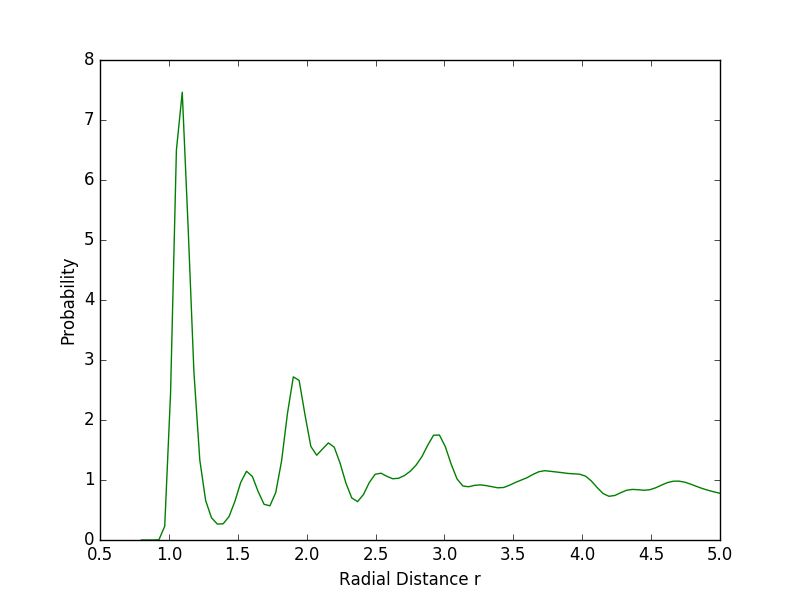
\includegraphics[width=\textwidth]{fig/meanRDF_T0d3.png}
\end{subfigure}
\hfill
\begin{subfigure}{0.3\textwidth}
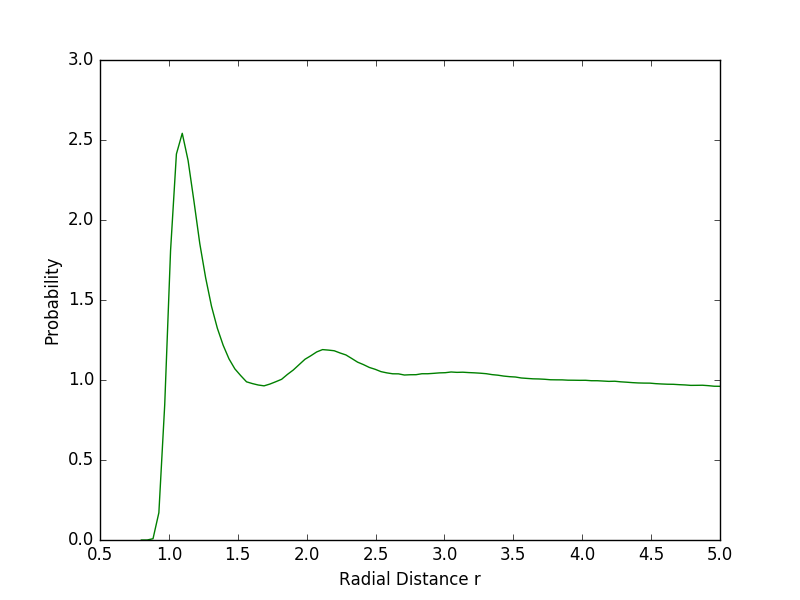
\includegraphics[width=\textwidth]{fig/meanRDF_T1d0.png}
\end{subfigure}
\hfill
\begin{subfigure}{0.3\textwidth}
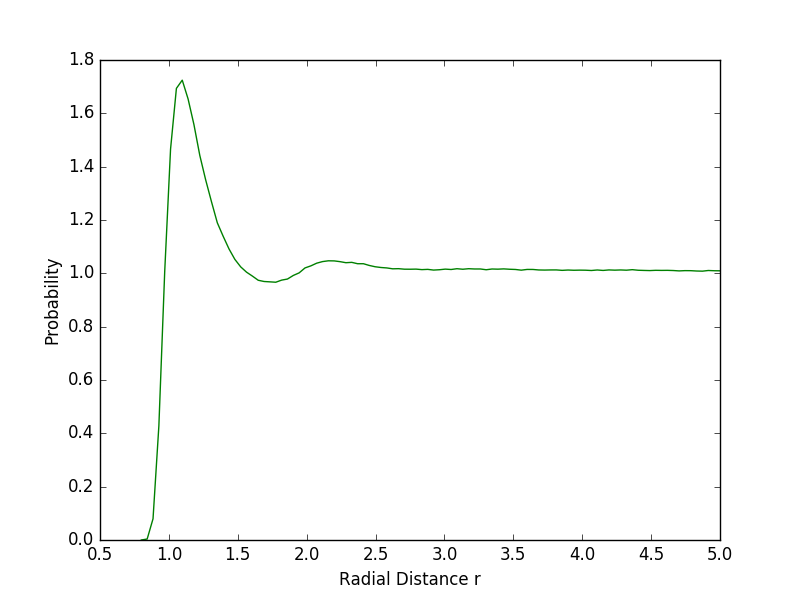
\includegraphics[width=\textwidth]{fig/meanRDF_T2d0.png}
\end{subfigure}
\end{figure}

